% !TEX root=./whitepaper.tex
\section{Log System Protocol}


The log layer of \projabbrev Storage provides decentralized storage service via a permissionless network of Storage Nodes.
These Storage Nodes collaboratively serve archived data,
where each node optionally specifies which portion of data it keeps in local storage.

\begin{figure}[H]
		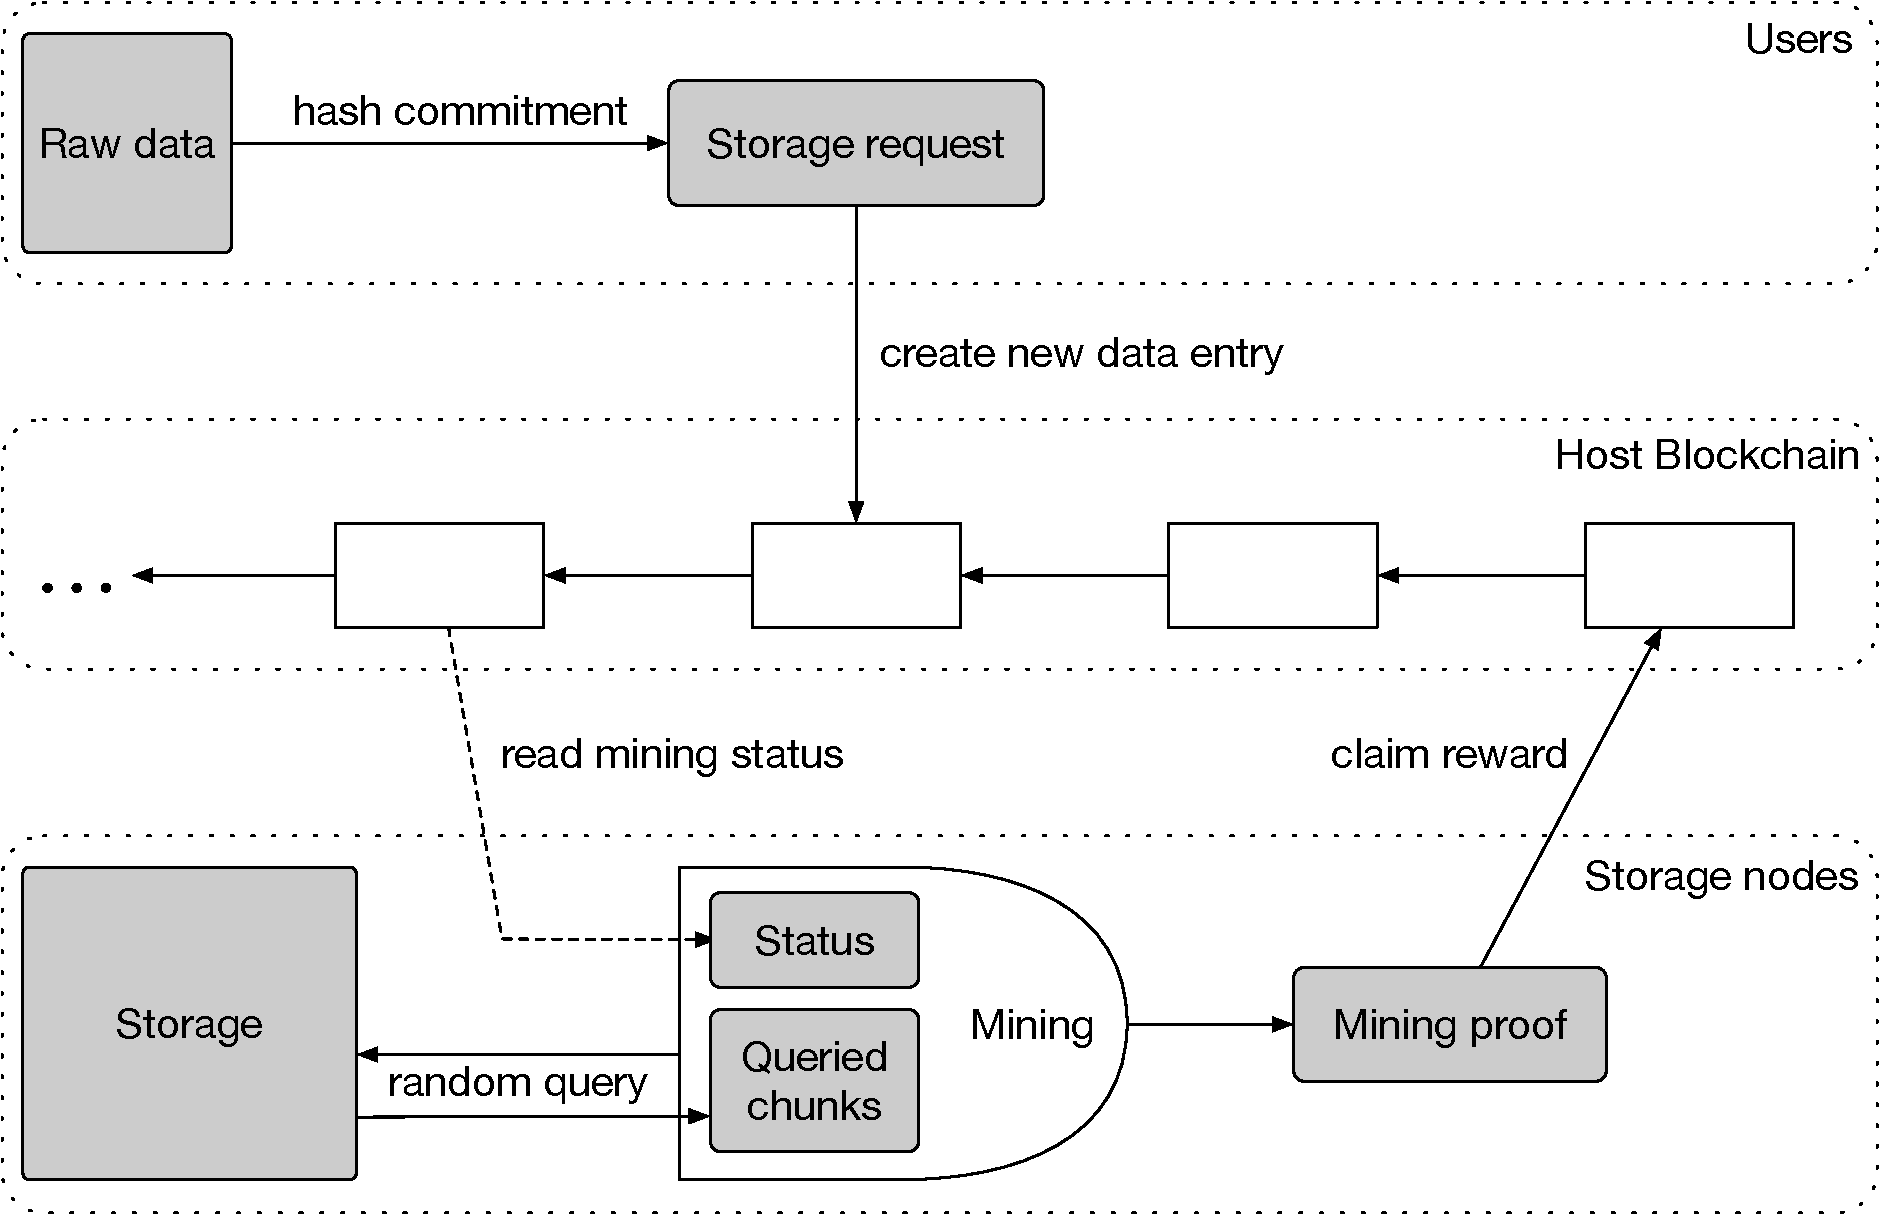
\includegraphics[width=\textwidth]{figure/protocol_overview.pdf}
		\caption{Overview of \projabbrev Storage protocol. Data creation and reward distribution are fully decoupled: users directly submit storage requests to the \projabbrev Storage contract deployed on host blockchain; Storage Nodes claim rewards by proving to the contract that they have the ability to answer random queries to archived data. \projabbrev tokens are handled in another isolated contract, which enables non-blocking token transfer.}
		\label{fig:overview}
\end{figure}

\subsection{Protocol Overview}

As a decentralized storage infrastructure, \projabbrev Storage prefers to improve existing blockchain ecosystems rather than build yet another ``storage service'' blockchain from scratch.

The storage state of \projabbrev Storage network is maintained in a smart contract deployed on an existing blockchain.
This contract is called the \projabbrev Storage \emph{contract} and the underlying blockchain is called the \emph{host blockchain} or \emph{host chain} for short.

The design of \projabbrev Storage network fully decouples data creation, reward distribution, and token circulation.

The \projabbrev Storage contract is responsible for data storage request processing, data entry creation, and reward distribution. 
Data storage requests are submitted by users who wish to store data in the \projabbrev Storage network,
where each request includes necessary metadata such as data size and commitments,
and it comes along with the payment for storage service.
Data entries are created for accepted data requests, keeping record of stored data while
reward distribution is handled independently through a mining process.
Storage Nodes submit mining proofs to the \projabbrev Storage contract to claim rewards for maintaining the \projabbrev Storage network.


The token circulation of \projabbrev is fully embedded into the host chain ecosystem,
as an ERC-20 token maintained by another contract called the \emph{\token ledger}.
% 
This embedding design brings significant advantages:
\begin{itemize}
	\item Simplicity: there is no need to maintain a full-fledged  consensus protocol,
	which reduces complexity and enables \projabbrev Storage to focus on decentralized storage service.

	\item Safety: the consensus is outsourced to the host blockchain, and hence inherits the security of the host blockchain. 
	Typically the more developed host blockchain would provide a stronger safety guarantee than a newly built blockchain.

	\item Accessibility: every smart contract on the host blockchain is able to access the original state of \project directly, without relying on some trusted off-chain notary. This difference is essential comparing to the projection of an external ledger managed by a third-party.

	\item Composability: \projabbrev tokens (\token) can always be transferred directly on the host blockchain, like any other ERC-20 tokens. 
	This is much more convenient than typical layer-2 ledgers, where transactions are first processed by layer-2 validators and then committed to the host chain after a significant latency.
	This feature empowers \projabbrev Storage stronger composability as a new lego to the ecosystem.
\end{itemize}


\subsection{Storage Granularity}

The log layer of \projabbrev Storage is updated (append-only) at the granularity of \emph{log entries}, 
where every entry is created by a storage-request transaction sent to the \projabbrev Storage contract.
The log layer is akin to a filesystem, with every log entry corresponding to a file.

The log system operates at the level of fixed-size \emph{sectors}, with each sector storing \sectorsize of data. 
To avoid one sector being shared by distinct log entries,
every log entry must be padded to multiple sectors.

The mining process of \projabbrev Storage requires proving data accessibility to random challenge queries.
To maximize the competitive edge of SSD storage, the challenge queries are set to the level of \chunksize \emph{chunks}, \ie 1024 sectors.
As every challenge query requires the miner to prove accessibility to a whole chunk of data, Storage Nodes would maintain data at the granularity of chunks. 

\subsection{Data Flow}
In \projabbrev Storage, committed data are organized sequentially.
Such a sequence of data is called a \emph{data flow}, which can be interpreted as a list of data entries or equivalently a sequence of fixed-size data sectors.
Thus, every piece of data in \project can be indexed conveniently with a universal offset.
This offset will be used to sample challenges in the mining process of \sproof.


The default data flow is called the ``main flow'' of \project, and it incorporates all new log entries (unless otherwise specified) in an append-only manner.

There are also specialized flows that only accept some category of log entries,
\eg data related to a specific application.
The most significant advantage of specialized flows is a consecutive addressing space, which may be crucial in some use cases. 
Furthermore, a specialized flow can apply customized storage price, which is typically significantly higher than the floor price of the default flow, and hence achieves better data availability and reliability.